\documentclass[
headings=optiontohead,              %allows double headers
12pt,                               %fontsize 
DIV=13,                             %koma script diveider amount. tells koma how much of the site can be written to
twoside=false,                      %if set to true, automatically formats as book style with different left and right pages
open=right,                         %starting page on twosided texts 
BCOR=0mm,                           %correction that accounts for the center of the pages being glued in
toc=bibliographynumbered            %bibliography gets a number and is listed in the table of contents
]{scrreport}

\usepackage[utf8]{inputenc}                     %correct encoding of output, technically not needed anymore
\usepackage[T1]{fontenc}                        %correct encoding of output, technically not needed anymore
\usepackage[english,ngerman]{babel}             %font that supports German and Englisch
\usepackage{upgreek}                            %non-cursive Greek letters
\usepackage[stretch=10,shrink=10,protrusion=true,expansion=true,final]{microtype}                          %prettier Blocksatz
\usepackage{hyperref}                           %links for everything
\usepackage{color}                              %allows for setting in different colors
\usepackage[autooneside=false,automark]{scrlayer-scrpage}%page-style with "Kolumnentitel" (title of current chapter is displayed at the top)
\usepackage{lmodern}                           %alternative font (better use libertinus)
\usepackage[sb]{libertinus}                     %use the font libertinus (needs to be installed from the web)
\usepackage[slantedGreek]{libertinust1math}     %math mode improvement for libertinus
\usepackage{siunitx}                            %physical units setting
\usepackage{icomma}                             %commas in lists get extra space if needed                        
\usepackage{amsfonts,amssymb,amstext,amsmath,amsthm} %better math mode (\mathrm and \text) and symbols
\usepackage{xspace}                             %works to improve own commands and provides "\xspace"-command, that puts a space if needed
\usepackage{ifthen}                             %more control over non-obligatory parameters
\usepackage[onehalfspacing]{setspace}           %control the spacing between lines and in enumeration lists
\usepackage[backend=biber, style=phys, biblabel=brackets]{biblatex}         %citations with "modern" backend and an physics-accepted citation style
\usepackage{graphicx}                           %work with graphics 
\usepackage{ragged2e}                           %ragged-commands (nicht-Blocksatz Einstellung)
\usepackage{pdfpages}                           %allows including of pdfs into this pdf
\usepackage{booktabs}                           %better table formatting
\usepackage{multicol}                           %allows for the definition of multi-columns in tables
\usepackage{multirow}                           %allows for the definition of multirow-tables instead of just multicolumn
\usepackage{tikz}                               %generate nice svg-pictures directly in latex
\usepackage{tikz-qtree}                         %generate trees with tikz
\usepackage{pgfplots}                           %better plotting with tikz
\usepackage{float}                              %provides the "H" option for forcing placement of a figure
\usepackage[section]{placeins}                  %provides the command "\FloatBarrier" to control the end of floatable regions for figures/tables
\usepackage{floatpag}                           %make it possible for float-pages to not have a page number
\usepackage{url}                                %sometimes needed by biblatex, technically no longer needed
\usepackage{minted}                             %nice code highlighting 
\usepackage{accents}                            %better control over accents
\usepackage{mathtools}                          %more math control possibilities
\usepackage[autostyle=true]{csquotes}           %context-sensitive-quotes -> quotation marks that are set correctly for the context
\usepackage{enumitem}                           %better enumerations (e.g. continue)

\usepackage{lipsum}                             %Generate blind text lorem ipsum
\usepackage{blindtext}                          %Generate blind text documents (in German)

\clubpenalty10000                                   % Schusterjunge, orphan
\widowpenalty10000                                  % Hurenkind, Witwe
\displaywidowpenalty=10000                          % Make document obey stricter rules considering "schusterjungen" and "hurenkinder"
\renewcommand{\topfraction}{0.8}                    % allows for more chilled "text to image ratio" 
\renewcommand{\bottomfraction}{0.8}
\renewcommand{\textfraction}{0.1}
\renewcommand{\floatpagefraction}{0.8}

\renewcaptionname{ngerman}{\figurename}{Abb.}       %"Abbildung" becomes "Abb." in German
\setcapindent{0cm}                                  %useful if image captions have multiple lines. Removers indentation below "Abb."
\setlength{\parindent}{0cm}                         %removes indentation at start of new paragraphs

%bibliography slots are redefined/modified here
\DeclareFieldFormat{journaltitle}{\textsl{#1}\isdot}
\DeclareFieldFormat{titlecase}{{#1}}

%COLORS
\definecolor{dblue}{rgb}{0,0,0.5}
\definecolor{dred}{rgb}{0.5,0,0}
\definecolor{dgrey}{rgb}{0.5,0.5,0.5}

%overwrite the coma-script definitions
\addtokomafont{pagehead}{\normalfont\color{dgrey}}                  %overwrite the coma-script definitions
\addtokomafont{sectioning}{\rmfamily\color{dblue}\boldmath}         %rmfamily puts headings in "normal" "Serifenschrift" instead of "sans-serif"  boldmath ensures a bold math font in subscripts
\addtokomafont{captionlabel}{\bfseries\footnotesize}                %better Abb. format
\addtokomafont{caption}{\footnotesize}                          
                                  %another file that holds format information


\newcommand*{\fullref}[1]{\hyperref[{#1}]{\textit{\ref*{#1} \nameref*{#1}}}}
\newcommand*{\fullpage}[1]{\hyperref[{#1}]{Seite \pageref*{#1}}}
\newcommand*{\fullpages}[1]{\hyperref[{#1}]{Seiten \pageref*{#1}ff}}
\newcommand{\thickbar}[1]{\accentset{\rule{.6em}{.8pt}}{#1}}                                %another file that holds predefined commands

\graphicspath{{./images/}}      %custom paths for folders in that graphics can be found

\linespread{1.1}                        %line-spacing can be controlled here

\sisetup                                %setup for siunitx
{
detect-all,
locale=DE,                              %language setup for siunitx
range-phrase={ \text{bis} },            %word that is put into an si range
range-units = brackets,                 %better display of error ranges
per-mode=symbol-or-fraction,            %more dynamic frac usage in inline/displaymath mode
separate-uncertainty,                   %for better +- , \pm when including an error range 
}

\hypersetup
{
colorlinks=true,
linkcolor=dblue,            %deep blue linkcolor
urlcolor=dblue,             %deep blue linkcolor
citecolor=dblue,            %deep blue linkcolor
pdfauthor = {Jonas Kell},                                   %write details into the expanded file properties
pdftitle = {Seminar Softwareentwicklung mit Dev(Sec)Ops},                         
pdfkeywords = {dev-ops, seminararbeit, ci-cd, licenses, checking},            
pdfsubject = {Dev-Ops and License-Checking}                      
}

\pgfplotsset{compat=1.17}

\AtBeginDocument{
	\let\mathbb\relax
	\DeclareMathAlphabet\PazoBB{U}{fplmbb}{m}{n}
	\newcommand{\mathbb}{\PazoBB}
}       %more options to the \mathbb command

\setminted[]{
    xleftmargin=.2cm,
    xrightmargin=.2cm,
    frame=single,
    framesep=.25cm,
    linenos,
    tabsize=4,
    breaklines,
    breakafter=.,
    breakaftersymbolpre= ,
}           %configure the minted code-highlighting style

\addbibresource{Literatur.bib}              %initialize bibtex with correct file

%!START THE DOCUMENT

\begin{document}
\thispagestyle{empty}           %make sure title page ist not numbered or anything else
\newcommand{\authorI}{Jonas Kell}
\newcommand{\mailI}{jonas.kell@student.uni-augsburg.de}

%MODIFY HERE! ----------------------
\newcommand{\veranstaltung}{Seminar: Softwareentwicklung mit Dev(Sec)Ops}
\newcommand{\papertitle}{Seminararbeit - License Checker}
%-----------------------------------

\title{\papertitle}
\author{\authorname}


\begin{titlepage}
\color{darkgray}
\veranstaltung \\
Sommersemester 2021\\
Universität Augsburg\\

\color{black}



\begin{center}
    \vspace*{3cm}
    
    \Huge
    \textbf{\veranstaltung}
    
    \vspace{0.5cm}
    \huge
    \papertitle % Versuchstitel
    
    \vspace{0.5cm}
    \hrule height 0.07cm 
    \vspace{0.5cm}
    \fontsize{15}{30}\selectfont

    \authorI: \href{mailto:\mailI}{\mailI}
\end{center}

\vfill

\noindent
\fontsize{12}{30}\selectfont
\renewcommand*{\arraystretch}{1.2}
\Large
\begin{center}
    \begin{tabular}{rl}
        Studiengang: &B.Sc. Informatik\\
        Abgegeben am: &\today
    \end{tabular}
\end{center}
\renewcommand*{\arraystretch}{1.5}
\end{titlepage}
           %include title-page
\cleardoublepage                %make sure, that if double-page is active, to reset the double page counter
\pagestyle{scrheadings}         %puts current chapters title into the header in small grey font
\pagenumbering{roman}           %number the pages of the table of contents in roman numerals
\tableofcontents                %table of contents include
\cleardoublepage                %make sure, that if double-page is active, to reset the double page counter
\pagenumbering{arabic}          %number the pages of the main document in Arabic numerals

% After this, the redefinition of the "Kolumnentitel" takes place
\clearpairofpagestyles
\ihead{\leftmark}
\ohead{\Ifstr{\leftmark}{\rightmark}{}{\rightmark}}
\cfoot*{\pagemark}
% End of the "Kolumnentitel" redefinition

\chapter{Diskussion: Dev(Sec)Ops}

Diese Arbeit stellt den schriftlichen Teil des Seminars \emph{Softwareentwicklung mit Dev(Sec)Ops} dar, das im Sommersemester 2021 im Zuge des B.Sc. Informatik an der Universität Augsburg angeboten wurde.

Die Arbeit setzt sich zusammen aus drei Teilen: Einem allgemeinen ersten Teil, indem das Thema \emph{Dev(Sec)Ops} (im folgenden vereinfachend oft nur \emph{DevOps}) ohne besondere Vorgaben in einem generellen Diskurs behandelt werden soll. Einem zweiten Teil, in dem die im Seminar behandelten Werkzeuge, Anwendungen und Methoden in einem möglichst funktionalen Gesamtsystem modelliert werden. Und einem dritten Teil, der an die Präsentation, bzw. den Vortrag \emph{Compliance: License-Checker} des Autors anknüpft, der ebenfalls im Zuge des Seminars gehalten wurde und einige der dort präsentierten Punkte nochmals schriftlich ausführt.

\section{Warum Dev(Sec)Ops}

Um zu verstehen, warum es in der modernen Softwareentwicklung nahezu unerlässlich geworden ist auf \emph{Dev(Sec)Ops} zurückzugreifen, muss zunächst der Begriff an sich verstanden werden. \emph{Dev(Sec)Ops} ist eine Zusammensetzung aus drei Abkürzungen und steht für \emph{Development(Security)Operations}, also \emph{Entwicklung(Sicherheit)Betrieb} \cite{forcepointWhatDevSecOpsDefined}. 

Damit stellt DevOps ein Gerüst von Prinzipien dar, die ein Team bei der Entwicklung einer Anwendung über den ganzen Produktlebenszyklus (von der Entwicklung bis zum Betrieb) hinweg unterstützen. DevOps hat keine festgeschriebene Definition und ist keine Anleitung der man Schritt für Schritt folgen kann. Es ist vielmehr ein Sammelbegriff für verschiedene Denkweisen, Praktiken und Werkzeuge \cite{awsWasIstDevOps}.

Dabei haben alle der Methodiken gemein, dass durch sie eine Verkürzung der Reaktionszeit eines Entwicklerteams ermöglicht werden kann. 
Wie bereits erwähnt, erstreckt sich diese Suche nach Zeitersparnis über den gesamten Lebenszyklus einer Anwendung. So kann beispielsweise durch einen \emph{automatisierten Test} der bereits auf der Maschine des Entwickler ausgeführt werden kann, verhindert werden, dass ein Programmierfehler in die Produktionsumgebung vordringen kann. Dies wäre ein Beispiel für die \emph{Development} Stufe. Auf der anderen Seite lassen sich auch Verfahren betrachten, die der \emph{Operations} Stufe beigemessen werden können. Ein \emph{aktives Monitoring} einer Anwendung kann das Entwicklerteam sofort auf einen Ausfall eines Systems hinweisen. Im besten Fall können damit Fehler behoben werden, bevor sie beim Endnutzer zu Problemen führen. Ohne das Monitoring als DevOps Baustein, wird der Entwicklerstab im besten Fall erst herangezogen wenn die Menge an Beschwerden und Schadensmeldungen zu hoch wird, im schlechtesten Fall gar nicht. In keinem der letzten beiden Fälle ist dies für den Ruf eines Produktes zuträglich.

Durch diese hohe Reaktivität ist die DevOps Mentalität eng mit den Methodiken der \emph{agilen Entwicklung} verwandt \cite{haufe-lexwaregmbhcokgAgileMethodenDefinition}. In beiden Fällen ist es das Ziel möglichst \emph{agil}, also schnell und flexibel auf (sich verändernde) Anforderungen reagieren zu können.
Die agile Entwicklung stellt eine Sammlung von Organisationsformen dar, die ein flexibles und modernes Entwicklungsklima erzeugen. Sie zeichnen sich vor allem dadurch aus, dass das jedem Mitarbeiter individuell mehr Verantwortung und Vertrauen zukommt, die Teamgrößen kleiner werden, die Hierarchien flacher und die Release-Zeiten kürzer \cite{haufe-lexwaregmbhcokgAgileMethodenDefinition}. Dadurch wird die Produktivität des Teams gesteigert und es bleibt offen für Veränderungen. Eines der bekanntesten Beispiele für eine agile Methode ist \emph{Scrum}. Dieses fokussiert sich darauf, den Entwicklern Zeit zum ungestörten Arbeiten ohne Unterbrechungen zu geben und gleichzeitig die Produktivität und Abschlussrate hoch zu halten und das Ziel nicht aus den Augen zu verlieren \cite{froemlingAgileMethodenWas2021}.

Bleibt noch der dritte Teil der Definition, die \emph{Security}. Dabei ist die Idee, die IT-Sicherheit nicht als eigenständigen Abschnitt im Lebenszyklus des Projektes zu betrachten, sondern kollaborativ jeden mit in die gemeinsame Verantwortung zu ziehen, die Sicherheit \emph{während} jeder Phase mit in den Ablauf zu integrieren \cite{redheadWasIstDevSecOps}.

Letzter Begriff, der im Zusammenhang mit Dev(Sec)Ops einhergeht, ist der des \emph{CI/CD/CT}. Diese Reihe von Abkürzungen steht für \emph{Continuous Integration/Continuous Delivery/Continuous Testing} \cite{kinsbrunerHowMakeCI2018}. Damit bilden diese drei Komponenten die Teile der sogenannten \emph{Pipeline}, eine automatisiert ausführbare Sammlung von Werkzeugen und Skripten um den Code des Projektes bei Änderungen zu \emph{integrieren} (z.B. durch automatisierte Versionskontrolle, Buildprozesse und Coding-Style Überprüfungen), in die Staging- oder Produktionsumgebung \emph{auszurollen} (z.B. durch automatisches/inkrementelles Patchen auf dem Produktionsserver, kompilieren für verschiedene Betriebssysteme und Monitoring aktiver Applikationen) und in jedem Schritt des Prozesses möglichst kontinuierlich zu \emph{testen} (z.B. durch Unittests, Komponententests oder Sicherheitstests (Pentests)). 

Damit stellt das Dev(Sec)Ops einen Sammelbegriff für eine \emph{Entwicklungs-Kultur} \cite{kolblSoftwareentwicklungMitDev2021} dar, unter deren Schirm Prozesse, Technologien und Personen zusammenkommen. Dabei liegt diesen allen ein \emph{feedbackgesteuertes, reaktives} Modell zugrunde und damit kann dies als die zentrale Idee beziehungsweise Eigenschaft gesehen werden.

\section{Für wen ist Dev(Sec)Ops?}

Im folgenden Abschnitt soll eine grundlegende Frage beantwortet werden: \glqq Für wen ist die DevOps Kultur?\grqq{}. 
Ist es nur eine neuartige Erscheinung, oder etwas, dessen Prinzipien sich nur die marktführenden Riesenkonzerne zu Nutze machen können?

Die kurze Antwort wird der Leser bereits erahnen können: \glqq Für JEDEN!\grqq{}. Die ausführlichere, dafür aber auch zufriedenstellendere Antwort ist komplizierter. 

Warum die DevOps Kultur für jedes Entwicklerteam geeignet ist, hat zunächst eine ganz grundlegenden Ursache, die im ersten Abschnitt dargelegt wurde: Es gibt keine festen Regeln oder Vorgaben. Möchte man DevOps Kultur in sein Unternehmen oder Projekt einfließen lassen, so muss man keine Standards erfüllen, keine Mindestmaße erreichen. 
Man kann soviel oder wenig wie man möchte inkrementell einführen.
Zugegeben, manche Prozesse und Technologien werden in Kombination mächtiger als alleine, aber was nicht ist kann ja noch werden.
Und eine Umgebung, die bereits Vorteile durch einzelne Elemente eines DevOps Prozess genießt, ist in den meisten Fällen offener für weitere Elemente. 

Gerade die agilen Methoden \emph{Kanban} oder \emph{Scrum} \cite{froemlingAgileMethodenWas2021} gehören in den heutigen Zeiten zum Quasi-Standard, was das Projektmanagement angeht. Kaum ein neues Projekt kann heutzutage noch strikt nach dem Wasserfallmodell durchgeführt werden \cite{tutorialspointSDLCWaterfallModel}. Zu unvorhersehbar sind die Entwicklungen des Software-Marktes und zu gering die verfügbare Zeit für Planung.
Ideen verwerfen und iterativ testen zu können triumphiert in den meisten Anwendungsfällen, da es keine \glqq perfekten\grqq{} Lösungen gibt.
Durch die hohe Zahl an Frameworks und Drittanbieter-Paketen gibt es oft viele verschiedene Lösungsstrategien für ein Problem.
Oft ist es also gar nicht möglich, im Voraus die \glqq ideale\grqq{} Lösung zu kennen oder gar zu planen. An einem iterativen Entwicklungsansatz führt also kein Weg vorbei.

Neben den Punkten \emph{inkrementeller Adaption} und \emph{agiler Methoden} stellt allerdings der dritte hier aufgeführte den wichtigsten dar: die Werkzeuge.
CI/CD Werkzeuge können bereits mit kleinem Aufwand große Kosten- und Zeitersparnis verursachen. 
Betrachte man das einfache Beispiel: Automatisches Ausrollen in die Produktionsumgebung \cite{sonBeginnerGuideBuilding2019}. 
Diese Aufgabe ist oft simpel und mit wenigen Kommandozeilen-Befehlen erledigt. Allerdings ist die Aufgabe repetitiv (Ausrollen bei jedem Release, auf mehreren Servern), mitunter Zeitaufwändig (Lange Build-Zeiten / Downloads) und unsicher (wenn jeder Zugriff auf die Produktionsumgebung hat, ist dies ein Sicherheitsrisiko).
All dies macht den Prozess fehleranfällig bei manueller Durchführung, jedoch ideal für das Ausführen durch eine Maschine. 
Der initiale Mehraufwand durch die Konfiguration der Werkzeuge wird in der Regel bereits nach wenigen Zyklen ausgeglichen sein. 

Es lässt sich also zusammenfassend sagen, dass jedes Element aus dem Bereich der DevOps-Kultur ein Team bereichern kann, ohne es dabei einzuschränken.
Da es also praktisch nur Vorteile mit sich bringt, eignet sich DevOps im Prinzip für jeden.

\chapter{Der \glqq ideale\grqq{} Dev-Sec-Ops Prozess}

\section{Welche Werkzeuge kommen zum Einsatz?}
\section{Wie ordnet man seine Pipeline am besten an?}
\chapter{Dev(Sec)Ops Werkzeug: License Checker}

Im letzten Kapitel wird auf eine Anforderung des begleitenden Vortrages \emph{Compliance: License-Checker} eingegangen. 
Im Zuge des Seminars sollten Nachforschungen zu einem ausgewählten Bestandteil des DevOps Prozesses angestellt werden. 
In diesem Fall wurde als Thema die \emph{License-Compliance} gewählt, also das Aufbauen unternehmensinterner Richtlinien und Methoden um bei der Arbeit mit Fremdsoftware die Lizenz Bestimmungen einzuhalten \cite{validatisComplianceDefinitionBedeutung} \cite{haufe-lexwaregmbhcokgBedeutungComplianceFuer}.


\begin{sloppypar}
Neben der Behandlung des Themas Lizenzen, war es integraler Bestandteil der Aufgabe einen Vergleich zwischen Software-Werkzeugen vorzunehmen. Diese Werkzeuge sollen das \mbox{(Entwickler-)Team} bei der Arbeit mit Lizenzen unterstützen. Und somit als Bestandteil der DevOps-Pipeline dazu beitragen die rechtlichen Anforderungen gewährleisten zu können.
\end{sloppypar}

\section{Auswahl des geeignetsten Werkzeugs}

Im Vortrag wurde ein Vergleich zwischen vier Werkzeugen vorgenommen: Die \glqq Open Source Security Platform\grqq{} \emph{Snyk} \cite{snykLicensingComplianceManagement}, das \glqq Open Source License Compliance Management Tool\grqq{} \emph{Fossa} \cite{fossaOpenSourceLicense}, das in der Versionskontrolle \emph{GitLab} integrierte Tool \emph{License Compliance} \cite{gitlabLicenseComplianceGitLab} und der \emph{Open-Source Ansatz}, einem Adapter für die Integration bereits existierender Lizenz-Überprüfungs\-werkzeuge in eine GitLab Pipeline \cite{kellOpenSourceLicenseChecker2021}.

Verglichen wurde nach mehreren Parametern. Eine tabellarische Übersicht ist auf \fullpage{anhang:tabelle} gegeben. Die Informationen auf dieser Tabelle stammen allesamt aus den Quellen \cite{snykLicensingComplianceManagement} \cite{fossaOpenSourceLicense} und \cite{gitlabLicenseComplianceGitLab}. Der Open-Source Adapter wurde speziell für dieses Seminar geschrieben. Er nutzt dabei zwei Open-Source Pakete \cite{glassNPMLicenseChecker} und \cite{bauernfeindComposerLicenseChecker}.

Die Entscheidung, welches der Werkzeuge das geeignetste ist, häng stark von den Gegebenheiten in der betrachteten Organisation ab. 
Für große Firmen sind die eigenständigen Plattformen Fossa und Snyk vermutlich die beste Wahl. Ab einer bestimmten Unternehmensgröße fallen einige tausend Dollar Kosten pro Monat wenig ins Gewicht. Diese werden schnell durch die Vorteile, wie hohe Regelkomplexität, Vorkonfiguration und Support aufgewogen. 
Snyk bietet die Lizenz-Analyse nur in den höheren Bezahlstufen an, verlangt also für alle für diesen Zweck geeigneten Anwendungsformen einen von der Entwicklerzahl abhängigen Preis. Da die Lizenz-Analyse nur Nebenfeature zu sein scheint, rentiert sich Snyk vermutlich nicht für den Zweck der Lizenzverwaltung allein, bietet aber ein starkes Ökosystem mit mehreren Werkzeugen, sollte das Angebot möglicherweise schon zu anderen Zwecken wahrgenommen werden.

Fossas Angebot bringt den Vorteil einer fähigen kostenfreien Version. Durch den Verzicht auf u.a. Verwaltungsoperationen bekommt man Zugriff auf einen Lizenz-Scanner mit hoher Konfigurierbarkeit und hochwertigen Voreinstellungen. Auch die Darstellung in der eigenen GUI ist übersichtlich. Die Möglichkeit die Werkzeuge lokal auf den Entwicklermaschinen oder eigenen Servern laufen zu lassen und nur die Ergebnisse in das Dashboard hochzuladen ermöglicht es, Analysen vorzunehmen ohne Fossa Zugriff auf den Code zu gegeben. Sollte man sich für die kostenpflichtige Version entscheiden ist diese allerdings direkt teurer, als die \emph{Team}-Stufe von Snyk.

Beide Plattformen lassen sich schnell mit Projekten aus einem GitLab-Repository betreiben, jedoch erfordert die Rückintegration in die GitLab Oberfläche auf den ersten Blick einen höheren Aufwand.

Mit genau diesem Argument besticht das integrierte Werkzeug von GitLab. Für Organisationen, die bereits stark auf GitLab-Pipelines setzen, ist das Aufsetzten dieses Analysetools mit wenigen Schritten getan und es ist vollständig in GitLabs Oberfläche integriert. Die Analyse ist solide, jedoch weniger stark konfigurierbar. Da in den meisten Fällen die Lizenz-Analyse allerdings ohnehin von im Thema Recht geschulten Mitarbeitern überprüft werden muss, ist es mitunter schon ausreichend, wenn das Werkzeug die Lizenzen auflisten kann und Alarm schlägt, wenn ein einfacher Regelfilter durch einen Änderung verletzt wird. Beides kann das GitLab interne Werkzeug problemlos liefern. 
Für sehr kleine Firmen oder Projekte ist schade, dass die vielseitigen Analysefunktionen nur in der \emph{Ultimate}-Version von GitLab zur Verfügung stehen. Diese ist für sich gesehen teurer, als sowohl die Angebote von Snyk und Fossa. Jedoch erlangt man durch die \emph{Ultimate}-Version Zugriff auf das komplette Angebot von Premium GitLab Funktionen. Dies ist für Firmen ab mittlerer Größe ohnehin beinahe unerlässlich, wenn GitLab als Hauptversionskontrollsystem genutzt wird. 

Zuletzt soll mit der Open-Source Variante ein direkter Ersatz für das GitLab-Werkzeug vorgestellt werden. 
Beinahe jeder Paketmanager bietet Lizenz-Analyse direkt oder mit einem Open-Source Paket. Diese sind lediglich nicht einer Pipeline Struktur automatisiert. 
Die wenigsten dieser Pakete formatieren leider ihre Ausgabe so, dass sie von GitLab analysiert werden kann. Mit Hilfe kurzer Shell-Skripte, lässt sich die Ausgabe der meisten Werkzeuge allerdings schnell in das gängige JUnit-Format \cite{ibmJUnitStandard} übersetzen. Dies integriert die Fähigkeiten der Open-Source Werkzeuge direkt in die Oberfläche von GitLab und bietet dazu das Überprüfen von einfachen \emph{Erlaubt-} oder \emph{Verboten-Filtern}.

Zusammengefasst lässt sich sagen: Kleine Unternehmen können mit etwas Aufwand für ihre Projekte die kostenlose Variante zum Einsatz bringen. Die anderen Werkzeuge rentieren sich für einzelne Projekte selten. Besteht bereits ein GitLab-Ultimate Zugang, so bietet dieser die schnellste und einfachste Lizenz-Analyse mit der besten Integration. Ist man Teil einer großen Organisation hohen Entwicklerzahlen und vielen Projekten, so werden die Angebote von Fossa oder Snyk irgendwann unerlässlich, um die Qualität der produzierten Software garantieren zu können.


\section{Inbetriebnahme}

Der finale Abschnitt soll eine Kurzanleitung für die Integration gängiger Open-Source Lizenz-Analysewerkzeuge in eine bestehende GitLab Pipeline sein.

Die Skripte zusammen mit einer Kurzdokumentation auf Englisch findet sich auch unter: \cite{kellOpenSourceLicenseChecker2021}. 

Für die Verwendung der Methode bedarf es einer funktionierenden GitLab Pipeline, mit entsprechenden \emph{Runnern}. Dies soll allerdings hier nicht näher erläutert werden und wird vorausgesetzt. 

Für jeden verwendeten Paketmanager wird ein eigenes Skript benötigt. Die Skripte werden in einem Ordner mit dem Namen \emph{license-checker} im untersten Projektordner platziert und richtig benannt. 
Vorkonfigurierte Skripte findet man zudem im Anhang. Für den Paketmanager \emph{npm} auf \fullpage{anhang:script-npm} und für den Paketmanager \emph{composer} auf \fullpage{anhang:script-composer}. 

Damit die Skripte in einer Pipeline richtig ausgeführt werden, muss ein entsprechender Job in der Pipeline definiert werden. Vorkonfigurierte Beispiele für Jobs, die die Skripte ausführen und die Ergebnisse an GitLab zurückgeben findet man auf Seite \fullpage{anhang:gitlabci} im Anhang.

In der Zeile \emph{script} müssen dann lediglich alle Lizenzen, die erlaubt werden sollen mit Semikolon getrennt zwischen die Hochkommata geschrieben werden.

%!LITERATURE AREA AND BIBLIOGRAPHY
\nocite{*} %cite all sources in the bibliography even if they aren't cited in the document
\printbibliography[title=Literaturverzeichnis] %bibliography with custom title
Die \autoref{fig:cicdprocess} wurde mit der Software \href{https://inkscape.org/}{Inkscape} erstellt.

%! Anhänge
\chapter{Anhänge}
    \section*{.gitlab-ci.yml} \label{anhang:gitlabci}
    \inputminted{yaml}{../code/.gitlab-ci.yml} 
    \newpage
    \section*{license-checker/npm-licenses.sh} \label{anhang:script-npm}
    \inputminted{bash}{../code/license-checker/npm-licenses.sh} 
    \newpage
    \section*{license-checker/composer-licenses.sh} \label{anhang:script-composer}
    \inputminted{bash}{../code/license-checker/composer-licenses.sh} 
    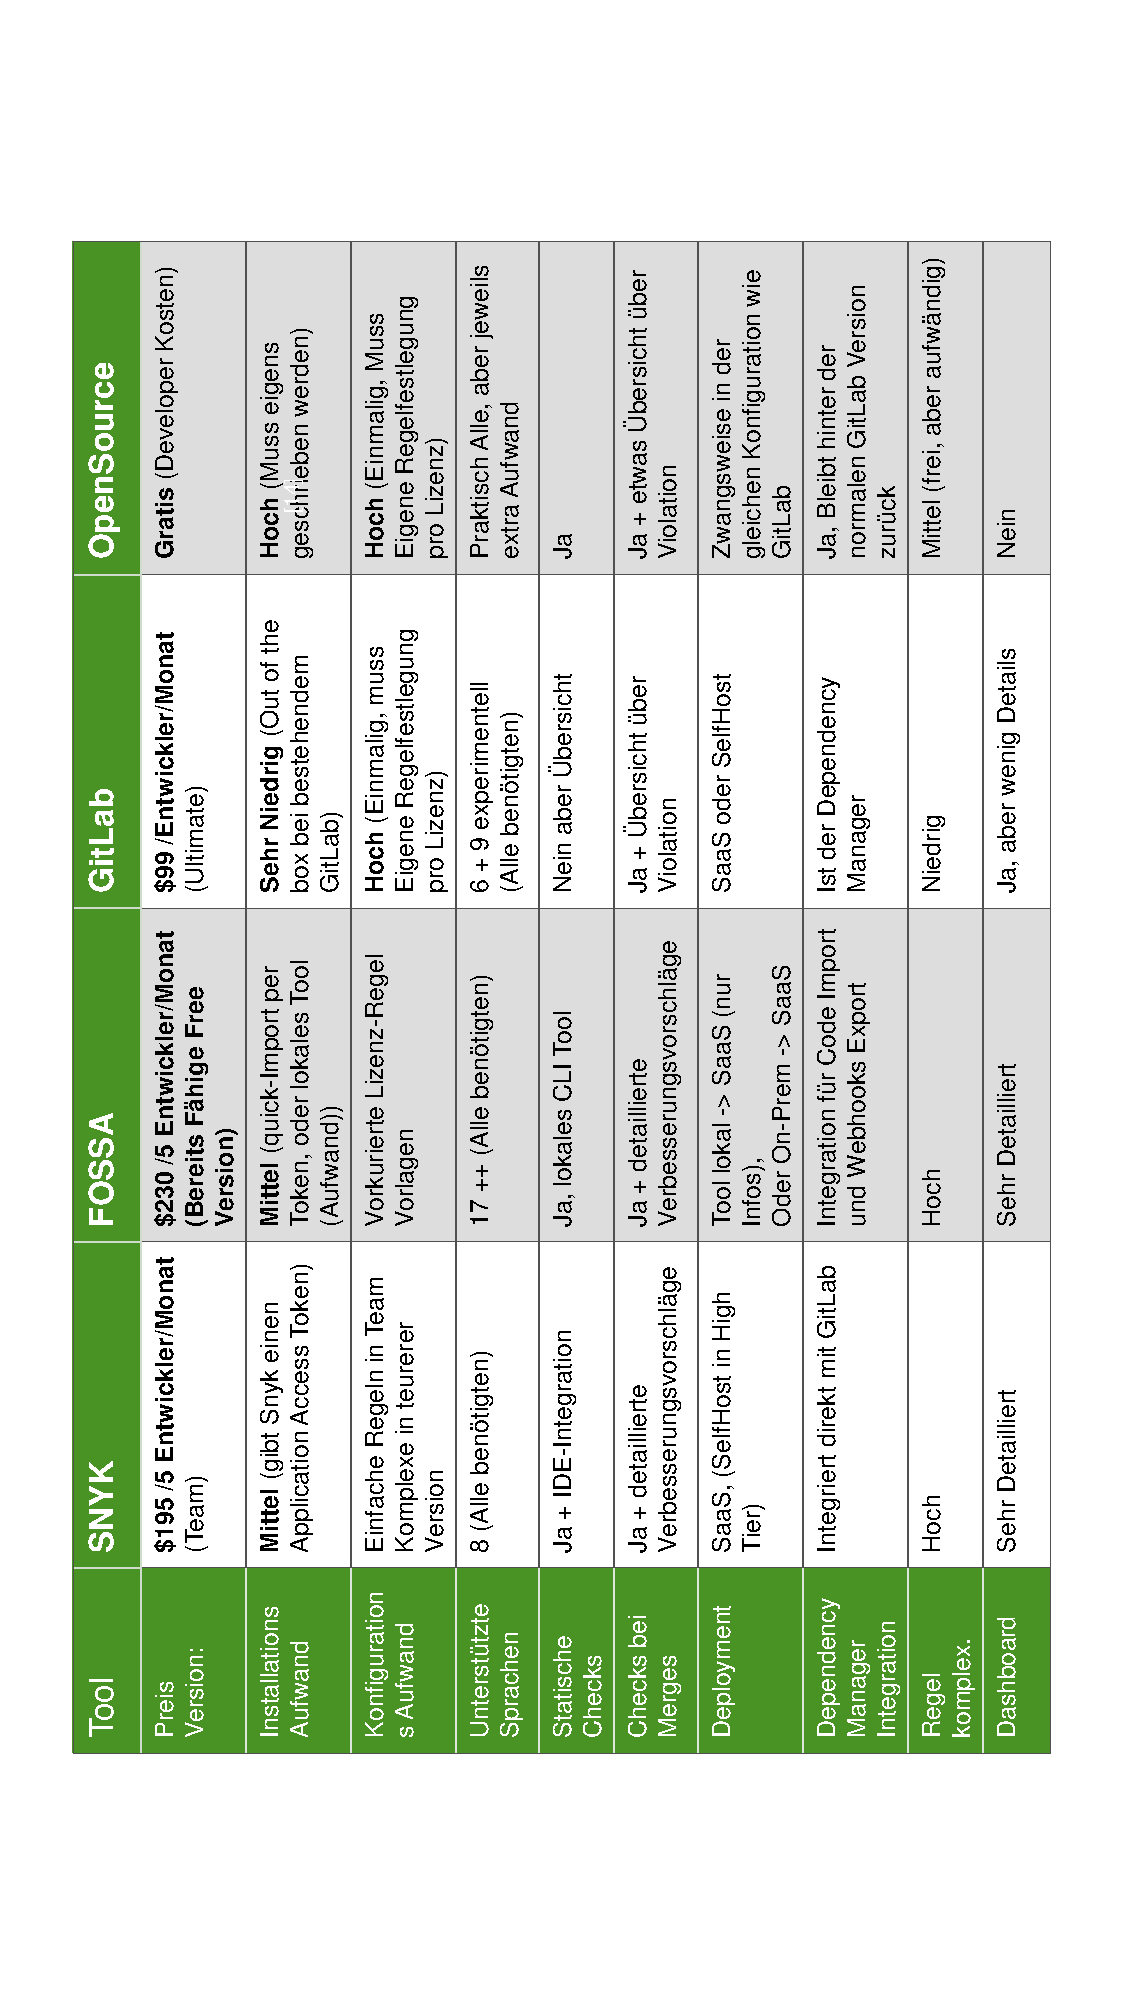
\includepdf[pagecommand={\section*{Tabelle: Vergleich Lizenzwerkzeuge} \label{anhang:tabelle}},landscape=false]{./AttachmentTable.pdf}
\end{document}